\documentclass[11pt]{article}
\usepackage[margin=1.1in]{geometry}
\usepackage{amsmath,amssymb}
\usepackage{graphicx}
\usepackage{booktabs}
\usepackage[hidelinks]{hyperref}

\newcommand{\dd}{\mathrm{d}}
\newcommand{\Pmod}{P_{\mathrm{mod}}}
\graphicspath{{../figures/}{../../square/figures/}{../../triangle/figures/}}

\title{Melt-pool uniformity optimization of a serpentine raster:\\
       exact per-segment Newton control with OTI derivatives}
\author{Notes on \texttt{melt\_pool\_demos/raster} (3DThesis + \texttt{cpp\_oti\_lib})}
\date{July 2026}

\begin{document}
\maketitle

\begin{abstract}
These notes document how the raster uniformity optimization works, end to end:
the semi-analytical forward model (3DThesis), how exact melt-pool
sensitivities are obtained from a single simulation using order-truncated
imaginary (OTI) numbers, how field derivatives become derivatives of the pool
\emph{dimensions} through the implicit function theorem, and the damped
per-segment Newton controller built on top. The demo holds the melt-pool
width and depth of a $1\times1$\,mm serpentine raster to a fixed target while
heat accumulates, reducing the width/depth coefficient of variation from
$9.7\%/7.1\%$ to $0.71\%/0.59\%$ in 49 simulations ($\approx$65\,s wall
clock, single process). Section~\ref{sec:square} extends the study to a
$10\times10$\,mm square at the published EBM-scale parameters of Stump and
Plotkowski's triangle experiment (150\,W absorbed, 3\,m/s,
$\sigma_{xy}=200\,\mu$m, IN718 at 1273\,K), where the pool is millimetres
long and merges across hatch lines. Judged on whole-build statistics ---
the beam-on fluctuation of the instantaneous pool dimensions --- the
controller cuts the pool-volume standard deviation $\approx4.5\times$
(from $0.077\pm0.024$ to $0.020\pm0.005$\,mm$^3$ at zero dwell) while
pinning the mean to the requested single-track setpoint; removing the
turnaround dwell trades a modestly tighter build (fusion-depth
$\sigma$ 4.4 vs.\ 6.7\,$\mu$m) against 26\% of build time.
\end{abstract}

\section{Problem statement}

A laser scans a $1\times1$\,mm square in a serpentine (boustrophedon) raster:
7 lines at speed $V=0.7$\,m/s with hatch spacing $H=0.15$\,mm, with a short
beam-off dwell at every turnaround. As the part heats up, a fixed-power beam
produces a melt pool that balloons --- both line to line (width grows
$97\to135\,\mu$m over the square) and within each line (each track starts
small on freshly solidified ground and swells toward its end).

The goal is \emph{geometric uniformity}: hold the pool's half-width $w$ and
depth $d$ at a fixed target $(w^\ast, d^\ast)$ for every control segment of
the path. Two controls are available per 0.5\,mm segment $i$:
\begin{align*}
  \Pmod{}_{,i} &\quad\text{--- power multiplier; segment power } Q_i = \Pmod{}_{,i}\, Q_{\mathrm{base}},\\
  \sigma_i     &\quad\text{--- lateral beam width (the Gaussian $\sigma_x=\sigma_y$ of the source).}
\end{align*}
Power scales how much material melts; beam width \emph{reshapes} the pool at
fixed power (wider beam $=$ same energy over a larger footprint $=$ broader,
shallower pool). Both knobs are needed: power alone cannot hold a fixed
$(w^\ast,d^\ast)$ pair once background preheat exists, because it only scales
the pool while the target also constrains its aspect ratio.

\section{Forward model: semi-analytical conduction (3DThesis)}
\label{sec:forward}

The thermal model is the adaptive-quadrature conduction solver of Stump and
Plotkowski~\cite{stump2019}, implemented in 3DThesis. Assuming constant
properties and pure conduction, energy conservation is
\begin{equation}
  \rho c\,\frac{\partial T}{\partial t} = k \nabla^2 T + \dot Q ,
  \label{eq:heat}
\end{equation}
which, for a volumetric Gaussian source moving along an arbitrary path on a
semi-infinite domain, has the transient integral solution (Nguyen et
al.~\cite{nguyen1999})
\begin{equation}
  T(\mathbf{x}_p, t) - T_0
  = \frac{2\eta Q}{\rho c\,(\pi/3)^{3/2}}
    \int_0^{t} \frac{1}{\sqrt{\phi_x \phi_y \phi_z}}
    \exp\!\left(
      -\frac{3x(t')^2}{\phi_x}
      -\frac{3y(t')^2}{\phi_y}
      -\frac{3z(t')^2}{\phi_z}
    \right) \dd t',
  \label{eq:nguyen}
\end{equation}
with $\phi_i = 12\alpha\,(t-t') + \sigma_i^2$ and
$\mathbf{x}(t') = \mathbf{x}_p - \mathbf{x}_b(t')$ the distance from the
evaluation point to the (piecewise-linear) beam position. Nondimensionalizing
on the lateral beam width $\sigma_{xy}$
\cite{stump2019},
\begin{equation}
  s=\frac{\alpha}{\sigma_{xy}^2}t,\qquad
  X=\frac{x}{\sigma_{xy}},\quad Y=\frac{y}{\sigma_{xy}},\quad Z=\frac{z}{\sigma_{xy}},\qquad
  \delta=\frac{\sigma_z}{\sigma_{xy}},
\end{equation}
puts the integrand into the universal form
\begin{equation}
  f(s'') = \frac{1}{(12 s''+1)\sqrt{12 s''+\delta}}
  \exp\!\left(-\frac{3\bigl(X^2+Y^2\bigr)}{12 s''+1}-\frac{3Z^2}{12 s''+\delta}\right),
  \label{eq:nondim}
\end{equation}
where $s''=s-s'$ is the conduction time available for heat deposited at $s'$
to diffuse. 3DThesis evaluates \eqref{eq:nguyen} by Gauss--Legendre
quadrature over sub-segments of the path history, with the two adaptive rules
of \cite{stump2019}: the segment size doubles as
$\Delta s'' = 2^{\lfloor \log_2 (s''+1)\rfloor}$ while the quadrature order
halves from 16 down to 2 (diffusion makes $f$ increasingly linear), and for a
moving source the node spacing is capped by
\begin{equation}
  \Delta s'' \;=\; \frac{\sqrt{(12 s''_n + 1)\,\ln\sqrt{2}}}{V^{*}},
  \qquad V^{*} = \frac{\sigma_{xy}\,\bar v}{\alpha},
  \label{eq:velocity-spacing}
\end{equation}
so that neighboring discrete sources overlap into a smooth field. The end
result: the temperature at any point is a \emph{finite weighted sum of
Gaussian contributions from quadrature nodes along the path history},
\begin{equation}
  T(\mathbf{x}_p) = T_0 + \sum_{n \in \text{nodes}}
     c_n\, \exp\!\left(
       -\,\frac{3\,(x_p - x_{b,n})^2}{\phi_{x,n}}
       -\,\frac{3\,(y_p - y_{b,n})^2}{\phi_{y,n}}
       -\,\frac{3\,(z_p - z_{b,n})^2}{\phi_{z,n}}
     \right),
  \label{eq:discrete}
\end{equation}
where for a node deposited at time $t'_n$ carrying power $Q_n$,
\begin{equation}
  c_n = \frac{2\eta\,Q_n}{\rho c\,(\pi/3)^{3/2}}\,
        \frac{w_n}{\sqrt{\phi_{x,n}\,\phi_{y,n}\,\phi_{z,n}}},
  \qquad
  \phi_{i,n} = 12\,\alpha\,(t - t'_n) + \sigma_i^2 ,
  \label{eq:cn}
\end{equation}
$w_n$ is the Gauss--Legendre weight of the node (times its sub-interval
length), $\alpha = k/\rho c$, and $t-t'_n$ its conduction time. This is
\eqref{eq:nondim} restored to dimensional form and summed by quadrature: the
Gaussian widths $\phi_i$ broaden with conduction time (diffusion), and $c_n$
carries the source strength together with the $1/\sqrt{\cdot}$ normalization.
The compact notation $\|\mathbf{x}_p-\mathbf{x}_{b,n}\|^2_{\Phi_n} \equiv
\sum_{i}(x_{p,i}-x_{b,n,i})^2/\phi_{i,n}$ abbreviates the exponent below. The
per-segment controls enter \eqref{eq:discrete} transparently: $\Pmod{}$ scales
$Q_n$ for the nodes of its segment, $\sigma$ enters $\phi_{x,n},\phi_{y,n}$
(3DThesis's path columns \texttt{Pmod}, \texttt{Wmod}), and the scan speed $v$
enters only through the node deposition times $t'_n$ (Section~\ref{sec:velderiv}).

Every optimization ``simulation'' below is one such solve on a small local
snapshot domain ($10\,\mu$m resolution, $0.5$\,mm buffer) placed at the end
of the truncated path, i.e.\ around the current pool.

\section{Exact derivatives in one pass: OTI numbers}
\label{sec:oti}

The optimizer needs derivatives of the pool dimensions with respect to the
controls. Rather than finite-differencing (3 simulations per Jacobian,
step-size tuning, subtractive cancellation), the OTI build of 3DThesis
computes them \emph{analytically in the same run}.

The scalar type of the entire solver is swapped
(\texttt{Real = oti::otinum<6,1,double>} from \texttt{cpp\_oti\_lib}): every
\texttt{Real} carries a value and six first-order partial derivative
coefficients,
\[
  T \;\longrightarrow\;
  \bigl(T;\ \partial_x T,\ \partial_y T,\ \partial_z T,\ \partial_Q T,\ \partial_\sigma T,\ \partial_v T\bigr),
\]
and every arithmetic operation propagates all six coefficients by the chain
rule, exactly, to machine precision. Truncation at order 1 means the cost is
a small constant factor over the plain \texttt{double} build (measured
$\approx 4.7\times$ for a seven-direction configuration), not the
$O(\text{re-runs})$ of finite differencing.

Three seeding sites define \emph{what} the derivatives mean:
\begin{itemize}
  \item \textbf{Evaluation point} ($x,y,z$): each grid point's coordinates are
        seeded in \texttt{Grid::Calc\_T}, so $T$ at that point carries its own
        spatial gradient $\nabla T$. This gradient is what converts field
        sensitivities into \emph{geometry} sensitivities
        (Section~\ref{sec:ift}).
  \item \textbf{Beam power} $Q$: seeded on the quadrature nodes of the
        \emph{current (last) path segment only}, per input watt. Hence
        $\partial T/\partial Q$ is the exact sensitivity to \emph{this
        segment's} power, with all history nodes carrying zero derivative.
  \item \textbf{Beam width} $\sigma$: likewise seeded on the current
        segment's effective lateral widths only.
  \item \textbf{Scan speed} $v$: seeded on the current segment's duration
        $\Delta t = L/v$. Unlike the four above, $v$ does not appear in the
        integrand at all; it reparametrizes the quadrature, and so needs the
        separate treatment of Section~\ref{sec:velderiv}.
\end{itemize}
The ``current segment only'' choice encodes the causality of the sequential
controller: segment $i$'s controls cannot change the already-executed history
$j<i$, and correspondingly the Jacobian entries are pure per-segment control
derivatives. This was verified against central finite differences (agreement
to $<1\%$, limited by FD truncation), including the negative control: an FD
perturbation of a \emph{history} segment's power does not reproduce the
$\partial T/\partial Q$ column, exactly as intended.

\paragraph{Differentiation under the quadrature.} It is worth being precise
about \emph{why} one hypercomplex pass suffices for $x,y,z,Q,\sigma$. Each of
these enters the discrete field \eqref{eq:discrete} \emph{only through the
summand} --- never through the node set, the weights, or the upper limit of
the sum. The nodes and weights are fixed by the adaptive schedule on the
real-valued path history, so seeding a parameter changes only the \emph{value}
each node contributes, not \emph{where} or \emph{how many} nodes there are.
Differentiation therefore commutes with the sum,
\begin{equation}
  \partial_p T = \sum_{n}
    \partial_p\!\left(c_n\, e^{-3\|\mathbf{x}_p-\mathbf{x}_{b,n}\|^2_{\Phi_n}}\right),
  \label{eq:diffundersum}
\end{equation}
the \emph{same} nodes and weights with each summand differentiated --- the
discrete analogue of differentiating \eqref{eq:nguyen} under the integral sign,
carried out operation-by-operation by the OTI arithmetic. This makes the three
``easy'' controls concrete: $Q$ is a linear prefactor of $c_n$, so
$\partial_Q T = (T-T_0)/Q$; the evaluation point enters only the exponent,
giving the spatial gradient $\partial_x T = \sum_n(\text{node}_n)\,
\bigl(-6\,(x-x_{b,n})/\phi_{x,n}\bigr)$ that Section~\ref{sec:ift} turns into a
geometry sensitivity; and $\sigma$ enters both the exponent (through
$\phi_x,\phi_y$ in $\Phi_n$) and the $1/\sqrt{\phi_x\phi_y\phi_z}$ normalization
in $c_n$, whose two chain-rule contributions the arithmetic combines
automatically. A control that lives in the integrand costs nothing but a slot.

\paragraph{Analytic verification.} Because these five enter only the summand,
their derivatives have closed forms --- a reference \emph{stronger} than finite
differencing, with no step size, truncation, or subtractive cancellation.
Writing $g_n = c_n\exp(-3\|\mathbf{x}_p-\mathbf{x}_{b,n}\|^2_{\Phi_n})$ for the
$n$-th node's contribution to \eqref{eq:discrete},
\begin{align}
  \partial_Q T &= (T-T_0)/Q, \label{eq:dQ}\\
  \partial_x T &= \sum_n g_n\,\frac{-6\,(x_p-x_{b,n})}{\phi_{x,n}}, \label{eq:dx}\\
  \partial_\sigma T &= \sum_n g_n\,\sigma\!\left(
        \frac{6\bigl[(x_p-x_{b,n})^2+(y_p-y_{b,n})^2\bigr]}{\phi_{x,n}^2}
        - \frac{2}{\phi_{x,n}}\right), \label{eq:dsig}
\end{align}
with $\partial_y T,\partial_z T$ analogous to \eqref{eq:dx}. Equation
\eqref{eq:dx} is the dimensional spatial gradient of \cite{stump2019}
(Appendix~B, their $G_x$); \eqref{eq:dsig} we derive here, and it is
straightforward precisely because $\sigma_x=\sigma_y=\sigma$ is a single
variable entering $\phi_x=\phi_y$ in \emph{both} the exponent and the
$1/\sqrt{\cdot}$ normalization (with $\sigma_z$ held fixed). Evaluated against a
stationary single-spot source --- one segment, so the OTI columns are the
\emph{full} derivatives and the path integral collapses to a one-dimensional
conduction-time integral computed independently by adaptive quadrature
(\texttt{scipy}) --- the OTI $\partial_x T,\partial_y T,\partial_z T,
\partial_\sigma T$ agree to $\sim\!10^{-6}$ relative (the solver's own forward
quadrature tolerance) and $\partial_Q T$ to machine precision
($\sim\!10^{-16}$ at strong signal), confirming the implementation and the
derived $\partial_\sigma T$ at once. Because $v$ instead reparametrizes the
sum, it has no such closed form and is validated separately below.

\subsection{Velocity: differentiating the quadrature itself}
\label{sec:velderiv}

Scan speed is the exception that proves the rule, and the reason it needed
work rather than a slot. At \emph{fixed} path geometry --- the raster must
still cover the part --- the current segment's speed $v$ appears nowhere in
the integrand; it sets the segment's \emph{duration} $\Delta t = L/v$ and,
through it, the time parametrization of the quadrature. Perturbing $v$ moves
the construction of the sum \eqref{eq:discrete}, not its summand, in three
coupled ways:
\begin{enumerate}
  \item the current segment's node \emph{conduction times} and \emph{weights}
        both scale with $\Delta t$ --- a node at path fraction $\xi$ sits at
        conduction time $(1-\xi)\Delta t$ with weight $\propto \Delta t$;
  \item the snapshot is taken at scan end, so the \emph{observation time}
        $t_{\mathrm{end}} = t_{i-1} + \Delta t$ itself moves with $v$;
  \item consequently \emph{every history node's} conduction time
        $t_{\mathrm{end}} - t'$ shifts, even though its own controls are frozen
        --- a channel with no analogue for $Q$ or $\sigma$.
\end{enumerate}
All three funnel through the single scalar $\Delta t = L/v$. Seeding it as the
sixth OTI direction, current-segment nodes take a multiplicative factor
$k = \Delta t(v)/\Delta t_0$ on both conduction time and weight (real part
$1$), and history nodes take an additive observation shift
$t_{\mathrm{shift}} = \Delta t(v) - \Delta t_0$ on their conduction time (real
part $0$); one pass then delivers $\partial_v T$ exactly. Appendix~\ref{app:vel}
carries out the matching closed-form derivation and shows term-for-term how
$k$ and $t_{\mathrm{shift}}$ reproduce it. In the plain-\texttt{double} build
$k=1$ and $t_{\mathrm{shift}}=0$ identically, so that path stays bit-for-bit
unchanged.

Validation against central finite differences: the field derivative
$\partial_v T$ agrees to $\sim\!0.02\%$ (median over the highest-signal grid
points) on both a single-track segment and a mid-raster segment, the latter
confirming the history channel (item~3) that a kinematics-only implementation
would miss; the depth sensitivity agrees to $<0.5\%$, and all signs are
physical (faster $\Rightarrow$ cooler, shallower, narrower). The half-width
finite difference shows larger apparent error, but only because it is read on
the $50\,\mu$m lateral grid: refining that grid collapses it toward the
grid-independent analytic $\partial_v w$, confirming the gap is the
marching-cubes width estimate, not $\partial_v T$.

Velocity also admits an \emph{analytic} check, and a stronger one: for a moving
source the temperature is still a one-dimensional integral over the deposition
time $t'$ (with $\mathbf{x}_{b}(t')$ the piecewise-linear beam position), whose
$v$-derivative --- $\dd T/\dd v = -(L/v^2)\,\dd T/\dd\Delta t$ with the three
channels derived in closed form in Appendix~\ref{app:vel} --- is evaluated
independently by adaptive quadrature. On a
straight multi-segment track, and at two different observation times, the OTI
$\partial_v T$ matches this reference to $\sim\!10^{-6}$ relative (the solver's
own forward-quadrature tolerance, away from the sign changes of $\partial_v T$),
together with $\partial_{x,y,z}T$ over the full path and $\partial_Q T,
\partial_\sigma T$ over the last segment --- i.e.\ every OTI direction, on the
raster-relevant moving geometry, verified against a closed-form reference.

\section{From field derivatives to pool-dimension derivatives}
\label{sec:ift}

The controller regulates pool \emph{geometry}, so the raw field derivatives
must be assembled into derivatives of the measured dimensions.

\paragraph{Measurement.} The pool boundary is the liquidus isotherm
$T = T_{\mathrm{liq}} = 1733$\,K, extracted from the snapshot grid by
marching cubes. The quantities of interest are taken at the extremal vertices
of that isosurface:
\[
  w = \tfrac12\,(y_{\mathrm{right}} - y_{\mathrm{left}}),
  \qquad
  d = -z_{\mathrm{bottom}},
  \qquad
  a = y_{\mathrm{right}} + y_{\mathrm{left}} \ \ \text{(centre offset)} .
\]

\paragraph{Implicit function theorem.} Let $p \in \{Q, \sigma\}$ be a control
and $y_e(p)$ the lateral position of an extremal edge point, defined
implicitly by
\begin{equation}
  T\bigl(y_e(p),\, p\bigr) = T_{\mathrm{liq}} .
\end{equation}
Differentiating,
\begin{equation}
  \frac{\dd y_e}{\dd p}
  = -\,\frac{\partial T/\partial p}{\partial T/\partial y}
  \;\Bigg|_{\text{at the edge point}} ,
  \qquad
  \frac{\dd z_b}{\dd p}
  = -\,\frac{\partial T/\partial p}{\partial T/\partial z}
  \;\Bigg|_{\text{at the bottom point}} .
  \label{eq:ift}
\end{equation}
At the \emph{widest} points of the isotherm the surface is tangent to the
$x$--$z$ plane, so the isotherm normal is aligned with $\pm y$ and the
one-dimensional relation \eqref{eq:ift} is the exact first-order edge
sensitivity (similarly $\pm z$ at the deepest point). Both numerator and
denominator are OTI coefficients interpolated (trilinearly) at the
fractional-index marching-cubes vertices; no additional simulation is
involved. Assembly is then linear:
\begin{equation}
  \frac{\dd w}{\dd p} = \frac12\!\left(\frac{\dd y_r}{\dd p}-\frac{\dd y_l}{\dd p}\right),
  \qquad
  \frac{\dd d}{\dd p} = -\frac{\dd z_b}{\dd p},
  \qquad
  \frac{\dd a}{\dd p} = \frac{\dd y_r}{\dd p}+\frac{\dd y_l}{\dd p}.
\end{equation}
These four numbers ($\dd w/\dd Q$, $\dd w/\dd\sigma$, $\dd d/\dd Q$,
$\dd d/\dd\sigma$) are the exact Jacobian of the control problem, obtained
from \emph{one} simulation.

\paragraph{Generic form.} The implementation
(\texttt{ExtractIsoSupportSensitivities}) does not hardcode the axes or the
control set. For an arbitrary unit direction $\mathbf e$, the isosurface
point extremal in $\mathbf e$ (the \emph{support point} $\mathbf x^\ast(\mathbf e)$)
has $\nabla T \parallel \mathbf e$, and the support value
$h(\mathbf e) = \mathbf e\cdot\mathbf x^\ast$ obeys
\begin{equation}
  \frac{\dd h(\mathbf e)}{\dd p}
  = -\,\frac{\partial T/\partial p}{\nabla T\cdot\mathbf e}
  \;\Bigg|_{\mathbf x^\ast(\mathbf e)},
  \label{eq:support}
\end{equation}
with the full gradient $\nabla T = (\partial_x T, \partial_y T, \partial_z T)$
taken from the snapshot's OTI columns and the controls $p$ \emph{discovered}
as every remaining \texttt{dT\_d}$\langle$\emph{name}$\rangle$ column. The
melt-pool QoIs are then just linear combinations,
$w = \tfrac12\bigl(h(+\hat y) + h(-\hat y)\bigr)$, $d = h(-\hat z)$,
$a = h(+\hat y) - h(-\hat y)$, and likewise for their derivatives. A 3DThesis
build with additional seeded design variables (velocity, material
properties, \ldots) is picked up by this layer with no code change.

\section{The sequential per-segment Newton controller}
\label{sec:newton}

Segments are optimized in path order (as the real process would execute
them). For segment $i$ with controls
$\mathbf{u} = (\Pmod{}, \sigma)$, define the residual
\begin{equation}
  \mathbf{r}(\mathbf{u}) =
  \begin{pmatrix} w(\mathbf{u}) - w^\ast \\ d(\mathbf{u}) - d^\ast \end{pmatrix},
  \qquad
  J(\mathbf{u}) =
  \begin{pmatrix}
    \partial w/\partial \Pmod{} & \partial w/\partial \sigma\\
    \partial d/\partial \Pmod{} & \partial d/\partial \sigma
  \end{pmatrix},
\end{equation}
where each evaluation of $\mathbf{r}$ \emph{and} $J$ is one OTI simulation of
the path truncated at segment $i$, with all history segments $j<i$ replaying
their already-optimized $(\Pmod{}_{,j}, \sigma_j)$ (sequential causality; the
per-segment width column carries $\sigma_j/\sigma_{\mathrm{base}}$).

A plain Newton step $\Delta\mathbf{u} = -J^{-1}\mathbf{r}$ is fragile here
(controls of different scales, near-singular $J$ when inherited heat
dominates, bound slamming), so the implemented step is a scaled, regularized
Gauss--Newton with safeguards:
\begin{enumerate}
  \item \textbf{Normalize}: residuals by the targets,
        $\tilde{\mathbf r} = \mathbf r \oslash (w^\ast, d^\ast)$; controls by
        characteristic scales $(1,\ 10\,\mu\mathrm{m})$.
  \item \textbf{Regularized step}: solve
        $(\tilde J^{\mathsf T}\tilde J + \lambda I)\,\Delta\mathbf{z}
         = -\tilde J^{\mathsf T}\tilde{\mathbf r}$ with Tikhonov parameter
        $\lambda = 2.5\times10^{-2}$ in scaled coordinates.
  \item \textbf{Trust region}: clip $\Delta\mathbf u$ componentwise to
        $(0.6,\ 10\,\mu\mathrm{m})$ per iteration.
  \item \textbf{Merit backtracking}: accept the trial only if the merit
        $\phi = \tfrac12\|\tilde{\mathbf r}\|^2$ decreases; otherwise halve
        the step ($\alpha = 1, \tfrac12, \ldots, \tfrac1{16}$). Each trial is
        itself an OTI simulation and is cached/reused as the next iterate's
        evaluation when accepted.
  \item \textbf{Bounds}: $\Pmod{} \in [0.05, 3]$,
        $\sigma \in [5, 60]\,\mu\mathrm{m}$. If no backtracked step improves
        the merit, the segment returns its \emph{best evaluated} state.
  \item \textbf{Warm starts}: the first segment after each turnaround uses
        the cool--slow turnaround seed. Each later segment on the same track
        starts from the immediately preceding converged control, encouraging
        smooth parameter transitions without carrying a line-end state across
        the turnaround.
\end{enumerate}
Convergence is declared at $\max_k |r_k|/\text{target}_k < 1\%$. In the demo
this takes 1--4 accepted iterations per segment ($\approx$2.3 on average) and
$\approx$3.5 simulations per segment including backtracking trials --- 49
simulations for all 14 controlled segments, about 65\,s wall clock in total
(single process; each local-domain OTI solve is $\approx$1.3\,s).

\section{Feasibility: three things the controller cannot fix}
\label{sec:feasibility}

Three physical constraints shape the problem setup; getting these wrong makes
the target unreachable no matter how good the optimizer is.

\paragraph{Turnaround dwell.} At $H=0.15$\,mm the return pass starts next to
the previous track's still-hot end. With an instantaneous turnaround the new
pool \emph{merges with still-liquid residue}; the measured width then
contains inherited melt that no control value can remove, and a fixed width
target is infeasible at track starts. The demo therefore inserts the
\emph{minimal} dwell such that the whole field has solidified when each new
track starts, found by bisection on $\max_{\mathbf{x}} T < T_{\mathrm{liq}}$
at the end of every dwell (at worst-case 60\,W power):
$t_{\mathrm{dwell}} = 1.234$\,ms.

\paragraph{Target selection.} A uniformity target must be a
\emph{sustainable fixed point} of the controlled process: reachable from a
fresh track start at moderate power \emph{and} holdable mid-line within the
control bounds. The demo uses the developed single-track pool (the last
segment of line~0, $w^\ast = d^\ast = 97.5\,\mu$m). Targeting the
heat-soaked centre-of-square pool instead (a snapshot of the \emph{defect},
not the goal) forces a $\sim$175\,W spike at every line start whose surplus
heat the following segments cannot control, and the schedule degenerates
into a spike-and-coast limit cycle.

\paragraph{Control-segment length.} The pool has thermal inertia: after a
segment's beam moves on, its superheated core keeps melting outward for
roughly $\tau \approx w^2/4\alpha \approx 0.4$\,ms. Control segments shorter
than this ($0.25$\,mm $=0.36$\,ms at $0.7$\,m/s) produce a period-2
``ping-pong'' --- alternate segments hit the target and the ones in between
catch their predecessor's afterglow. With $0.5$\,mm segments ($\approx$2
relaxation times) each segment reaches its own quasi-steady pool before it is
measured, and the cycling vanishes.

\section{Results}

\begin{table}[h]
\centering
\small
\begin{tabular}{lcccc}
\toprule
 & width CV (\%) & depth CV (\%) & $w$ range ($\mu$m) & $d$ range ($\mu$m)\\
\midrule
unoptimized (constant 60\,W) & 9.72 & 7.14 & 38.3 & 26.7\\
optimized ($\Pmod{},\sigma$ per segment) & \textbf{0.71} & \textbf{0.59} & \textbf{2.3} & \textbf{1.9}\\
\bottomrule
\end{tabular}
\caption{Melt-pool uniformity over the raster, measured on the 14 controlled
segments. 49 OTI simulations, $\approx$65\,s wall clock single-process.}
\label{tab:results}
\end{table}

The optimized schedule is smooth and interior: line~0 runs at the nominal
(60\,W, $\sigma=10\,\mu$m); once neighbour preheat exists the power settles
to $\approx$41--48\,W with $\sigma$ near 9.6--10\,$\mu$m
(Figure~\ref{fig:dims}).

MPI operation was verified separately: with the domain-decomposed 3DThesis
build the same optimization reproduces the serial schedule bit-for-bit
(rank snapshot slices must be re-sorted into grid order before measurement).
At this problem size MPI is \emph{not} faster ($\approx$1\,s solves; launch
and merge overhead dominates); it pays off on larger domains, where the same
build scales $\approx 2\times$ at 4 ranks.

\begin{figure}[h]
\centering
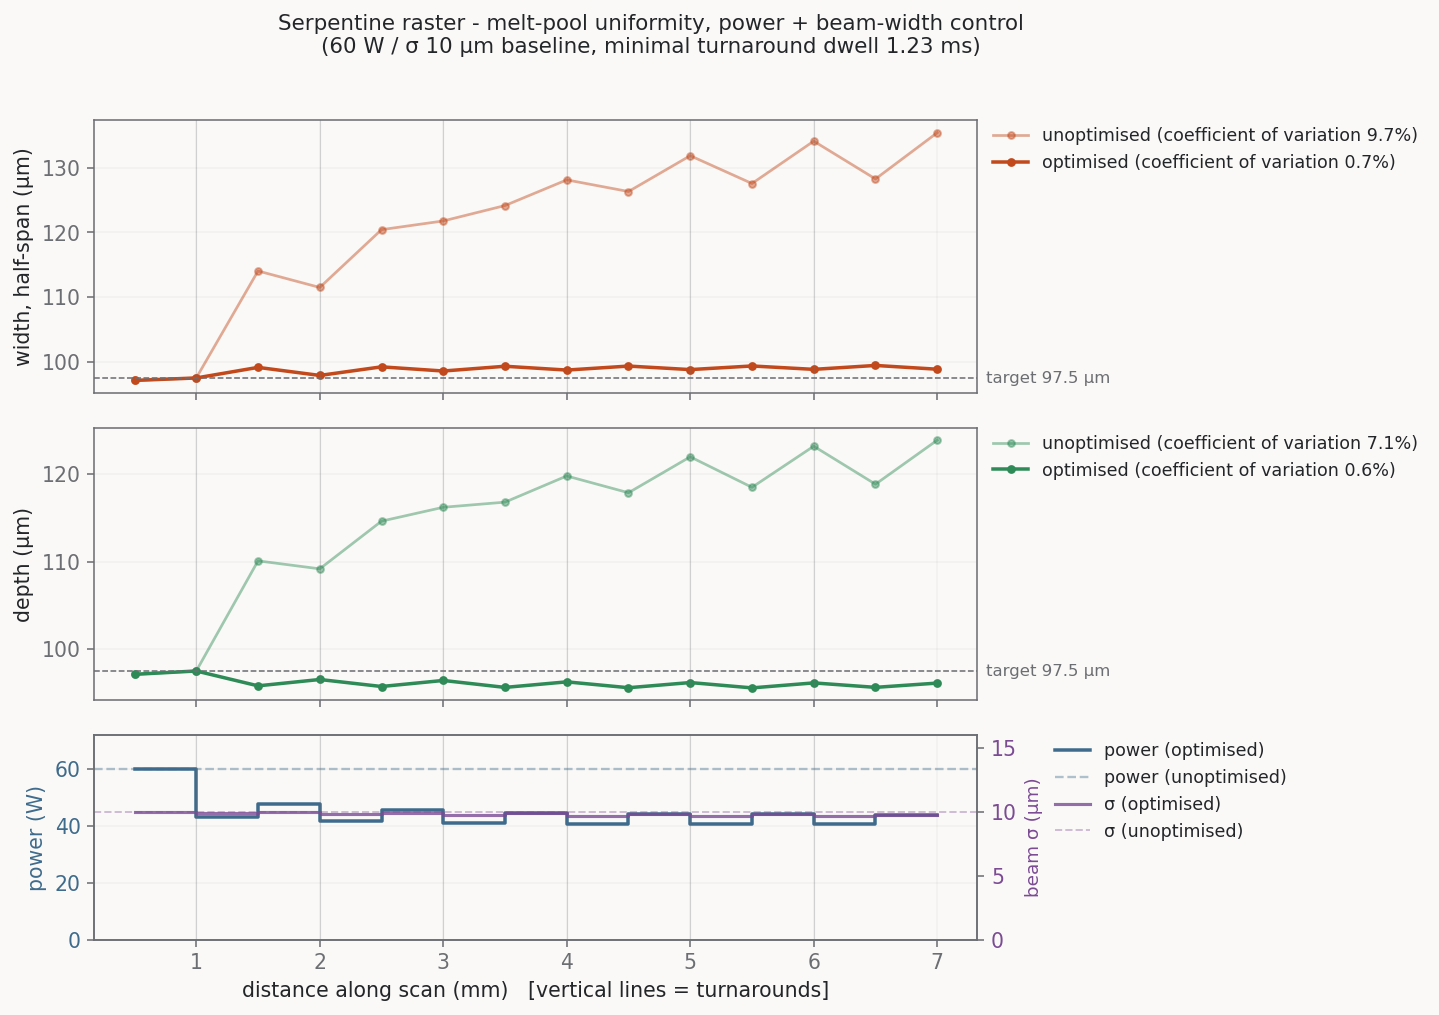
\includegraphics[width=\textwidth]{raster_dims.png}
\caption{Width and depth along the scan path, unoptimized vs.\ optimized,
with the optimized power and beam-width schedules (bottom panels).}
\label{fig:dims}
\end{figure}

\begin{figure}[h]
\centering
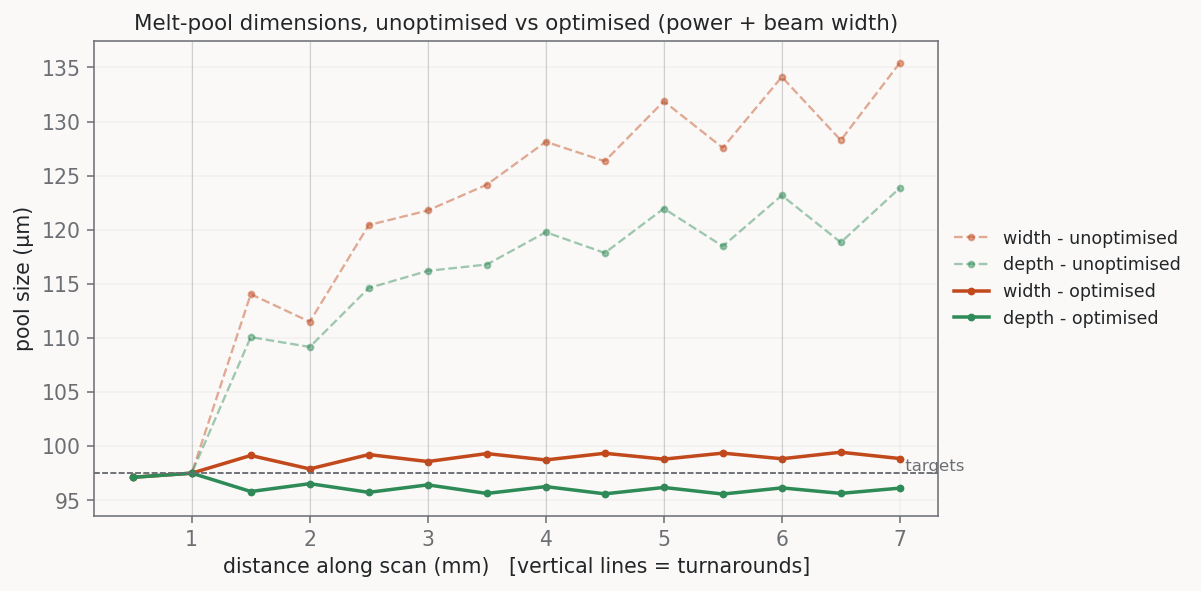
\includegraphics[width=0.8\textwidth]{raster_overlay.png}
\caption{All four dimension traces on one axis: the optimized width and
depth collapse onto the target while the unoptimized traces drift and
sawtooth.}
\label{fig:overlay}
\end{figure}

\section{Scaling up: a 10\,mm square at published EBM parameters}
\label{sec:square}

The raster demo above lives in a compact-pool regime: a $\sim$100\,$\mu$m
hemispherical pool, small against both the line length and the hatch. To
prepare the optimization of Stump and Plotkowski's triangle experiment
(their \S3.5), the study was repeated on a $10\times10$\,mm square at that
experiment's physics --- IN718 at $T_0=1273$\,K, $V=3$\,m/s,
$\sigma_{xy}=200\,\mu$m, $\sigma_z=10\,\mu$m, $Q=150$\,W absorbed,
$T_{\mathrm{liq}}=1610$\,K, hatch $H=0.1$\,mm
(\texttt{melt\_pool\_demos/square}; the same scripts drive the triangle
geometry). The square keeps the line length constant, so the process reaches
a statistically steady state that the triangle's shrinking lines never do.

\paragraph{Regime change.} A single-track calibration run sets the scales:
the developed pool is $2.05$\,mm long ($1.95$\,mm trailing), $0.30$\,mm
wide, and $60\,\mu$m deep, with a $0.55$\,ms post-beam solidification tail.
Because the beam ($\sigma_{xy}=200\,\mu$m) is wider than two hatch spacings,
the liquid spans many tracks laterally --- a melt \emph{front} rather than
discrete tracks. Everything resizes accordingly: control segments of 5\,mm
(two per line, $\geq 2$ pool-relaxation lengths), a measurement box
extending 7\,mm behind the segment end, and the target taken again from the
developed single track of line~0 ($w^\ast = 163.8\,\mu$m half-span,
$d^\ast = 63.3\,\mu$m on the snapshot grid).

\paragraph{Two dwell policies.} The published experiment scans
continuously, so zero dwell is studied alongside the raster demo's minimal
worst-case dwell. The minimal dwell --- bisected on the RDF event list with
the criterion \emph{no liquid cell anywhere at any line-start instant} ---
is $0.906$\,ms/turn, binding at a mid-square turn (the steady regime, unlike
the small raster where accumulation made the last turn binding), and adds
26\% to the build time. At zero dwell the field \emph{never} solidifies
between lines: every line start inherits $\approx 0.06$\,mm$^3$ of
still-liquid residue, about three single-track pools' worth. The target is
deliberately kept identical (the well-formed single-track pool, never the
heat-soaked one), and any resulting infeasibility is left to appear honestly
as bound-pinned segments rather than hidden by re-measuring. In the
continuous path the 0.1\,mm serpentine hops stay powered; they are excluded
from the control set and execute the controls of the segment they follow.

\paragraph{How the results are judged.} The controller regulates snapshot
dimensions at the 202 segment ends, but the part does not care about the
control grid, so results are reported on \emph{whole-build} statistics from
full solidification-tracked replays of the optimized schedules: the mean
and standard deviation of the \emph{instantaneous} pool depth, length, and
volume over every beam-on instant (50\,$\mu$s sampling from the RDF event
list). Beam-off dwell windows are excised --- a pool solidifying during a
designed dwell is the end of that pool's life, not process variation.
Fluctuations are quoted in absolute units rather than as CVs: the optimizer
shrinks the mean pool together with its spread, so relative measures hide
the reduction, and part defects (remelt geometry, microstructure gradients)
live in absolute units. The companion spatial view is the
\emph{fusion-depth map}: the deepest melt each interior $(x,y)$ column
attained over the entire build --- a max-attained quantity that cooling
never touches.

\begin{table}[h]
\centering
\small
\begin{tabular}{lccccc}
\toprule
beam-on mean $\pm\,\sigma$ & depth ($\mu$m) & length (mm) & lateral extent (mm) & volume (mm$^3$) & fusion depth ($\mu$m)\\
\midrule
zero dwell, unoptimized & $106 \pm 12.9$ & $4.24 \pm 1.23$ & $0.34 \pm 0.035$ & $0.077 \pm 0.024$ & $106 \pm 10.7$\\
zero dwell, optimized & $\mathbf{69 \pm 7.2}$ & $\mathbf{2.22 \pm 0.47}$ & $0.31 \pm 0.016$ & $\mathbf{0.020 \pm 0.005}$ & $67 \pm 6.7$\\
minimal dwell, unoptimized & $94 \pm 15.4$ & $3.40 \pm 1.36$ & $0.31 \pm 0.034$ & $0.054 \pm 0.021$ & $95 \pm 8.5$\\
minimal dwell, optimized & $\mathbf{64 \pm 8.7}$ & $\mathbf{1.99 \pm 0.55}$ & $0.30 \pm 0.026$ & $\mathbf{0.017 \pm 0.004}$ & $64 \pm 4.4$\\
\bottomrule
\end{tabular}
\caption{The 10\,mm square at the published parameters: whole-build pool
statistics (beam-on instants of the tracked replays) and the fusion-depth
map over interior columns. ``Lateral extent'' is the $y$-span of all liquid
--- at zero dwell this includes the neighbouring track's still-molten band
--- not the beam-frame track half-width the controller regulates. Each
optimization used $\approx$220 OTI simulations ($1.1$ per segment ---
sequential within-line warm starts let most segments converge on their first
evaluation) in $\approx$25\,min single-process. Depth statistics carry the
5\,$\mu$m $z$-grid quantization of these replays.}
\label{tab:square}
\end{table}

\paragraph{What the optimizer achieves.} The absolute pool fluctuation
drops $\approx2\times$ in depth, $2.5\times$ in length, and
$4.5\times$ in volume (Table~\ref{tab:square},
Figure~\ref{fig:square-traces}), while the mean is simultaneously pinned to
the requested setpoint (67/64\,$\mu$m attained vs.\ 63.3 requested; the
constant-power baselines run 50--65\% too deep). The residual fluctuation
is dominated by a once-per-line startup transient --- the pool briefly
overshoots to $\approx85\,\mu$m over the first 1--2\,mm of each line, where
the fresh track crosses its neighbour's still-hot end --- a sub-segment
feature invisible to a controller whose actions are constant per 5\,mm
segment and whose residual is evaluated after the transient has relaxed.
Regulating it needs sub-segment authority: a within-segment peak term in
the residual, graded segment lengths near the turns, or the velocity and
dwell controls of Section~\ref{sec:square}. As controller diagnostics (did
the Newton converge --- not part quality): the segment-end width/depth CVs
fall from $3.5/7.2\%$ to $0.12/0.21\%$ (minimal dwell) and $4.2/10.3\%$ to
$0.19/0.36\%$ (zero dwell), with \textbf{no segment pinned at a control
bound} in either policy --- the single-track target is feasible everywhere
on this geometry.

\paragraph{The price of zero dwell.} A genuine trade-off rather than a free
lunch in either direction: the dwell buys a modestly tighter build at part
level (fusion-depth $\sigma$ 4.4 vs.\ 6.7\,$\mu$m; beam-on volume
$\sigma$ 0.0044 vs.\ 0.0053\,mm$^3$) at the cost of $+26\%$ build time (428 vs.\
341\,ms). Both optimized schedules are smooth, interior, and line-periodic;
the zero-dwell schedule runs $\approx$5\,W cooler because inherited
background heat performs part of the melting, and it leaves $3.5\times$ less residual
liquid at line starts than the constant-power baseline ($0.017$ vs.\
$0.059$\,mm$^3$ mean) --- holding the target forces a cooler schedule,
which attacks the merged-pool defect indirectly.

\begin{figure}[h]
\centering
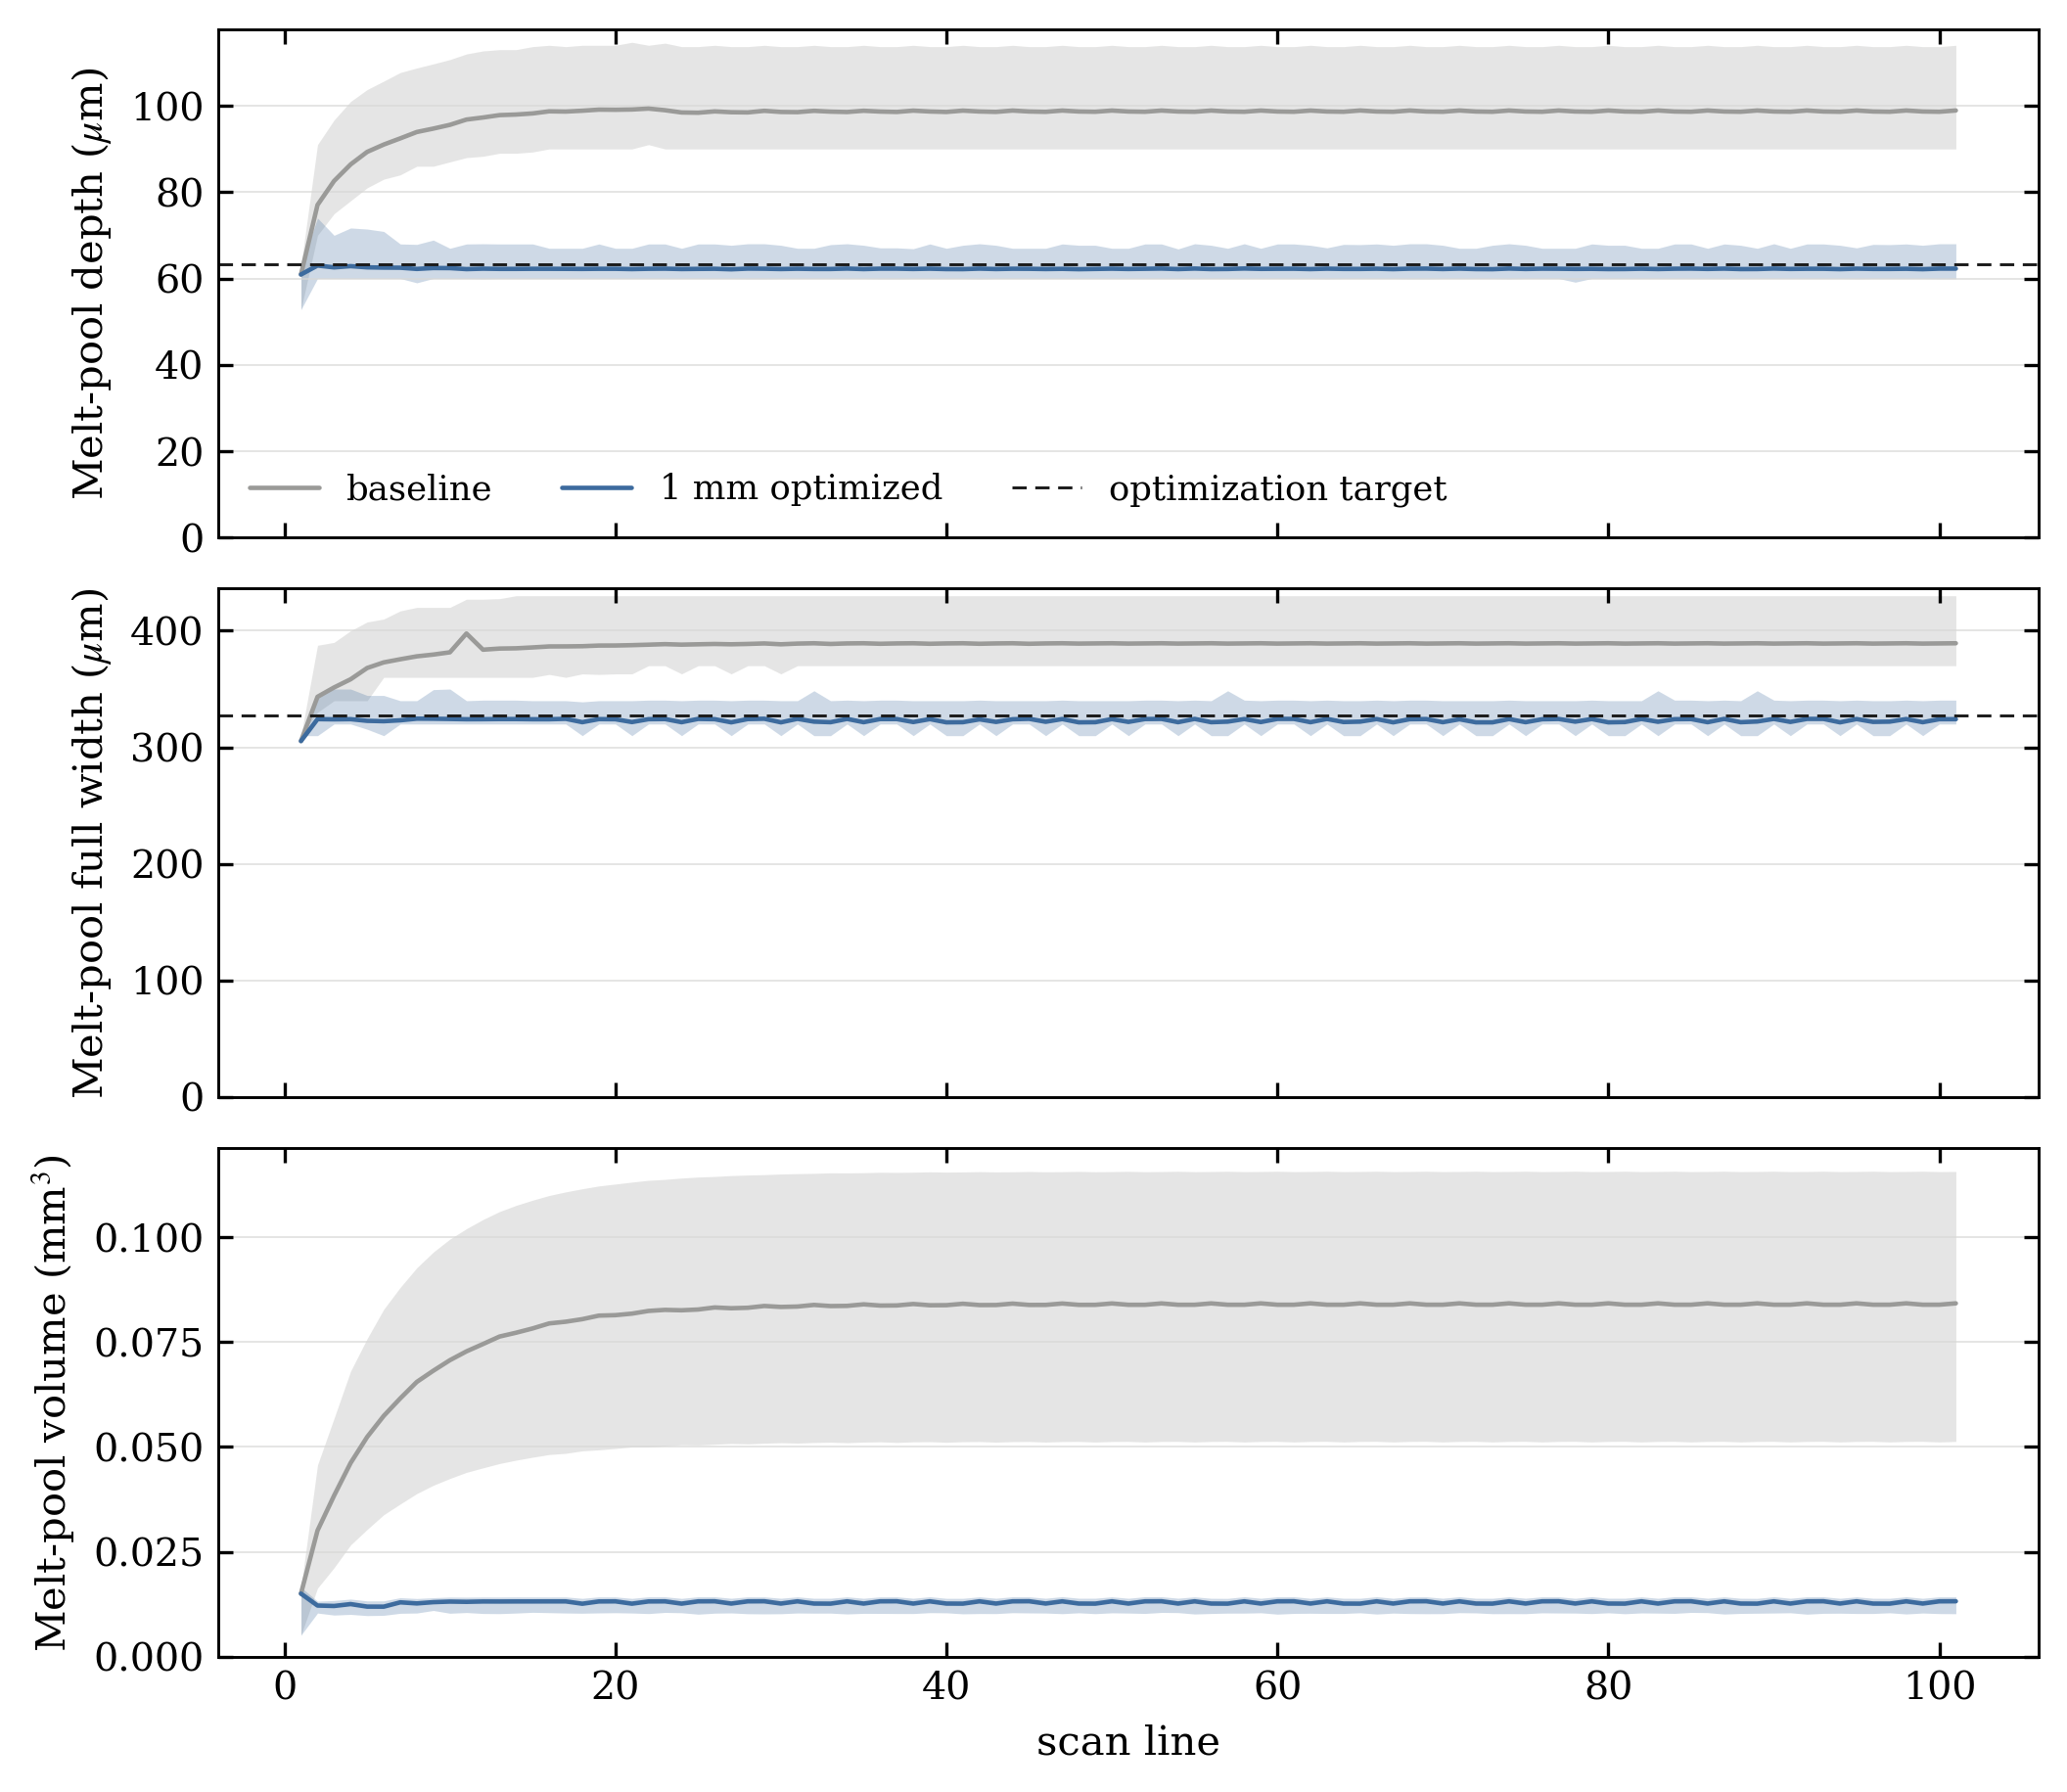
\includegraphics[width=0.95\textwidth]{square_traces_zero.png}
\caption{Per-line pool statistics of the zero-dwell square (RDF event
list, constant-power baseline vs.\ the replayed optimized schedule):
for each scan line, the mean (solid) and the 5th--95th percentile band
(shaded) of the instantaneous beam-on depth, volume, and length,
annotated per panel with the whole-build beam-on mean\,$\pm\,\sigma$
of Table~\ref{tab:square}. The bottom strip resolves three mid-build
lines in real time (marked in the depth panel).}
\label{fig:square-traces}
\end{figure}

\begin{figure}[h]
\centering
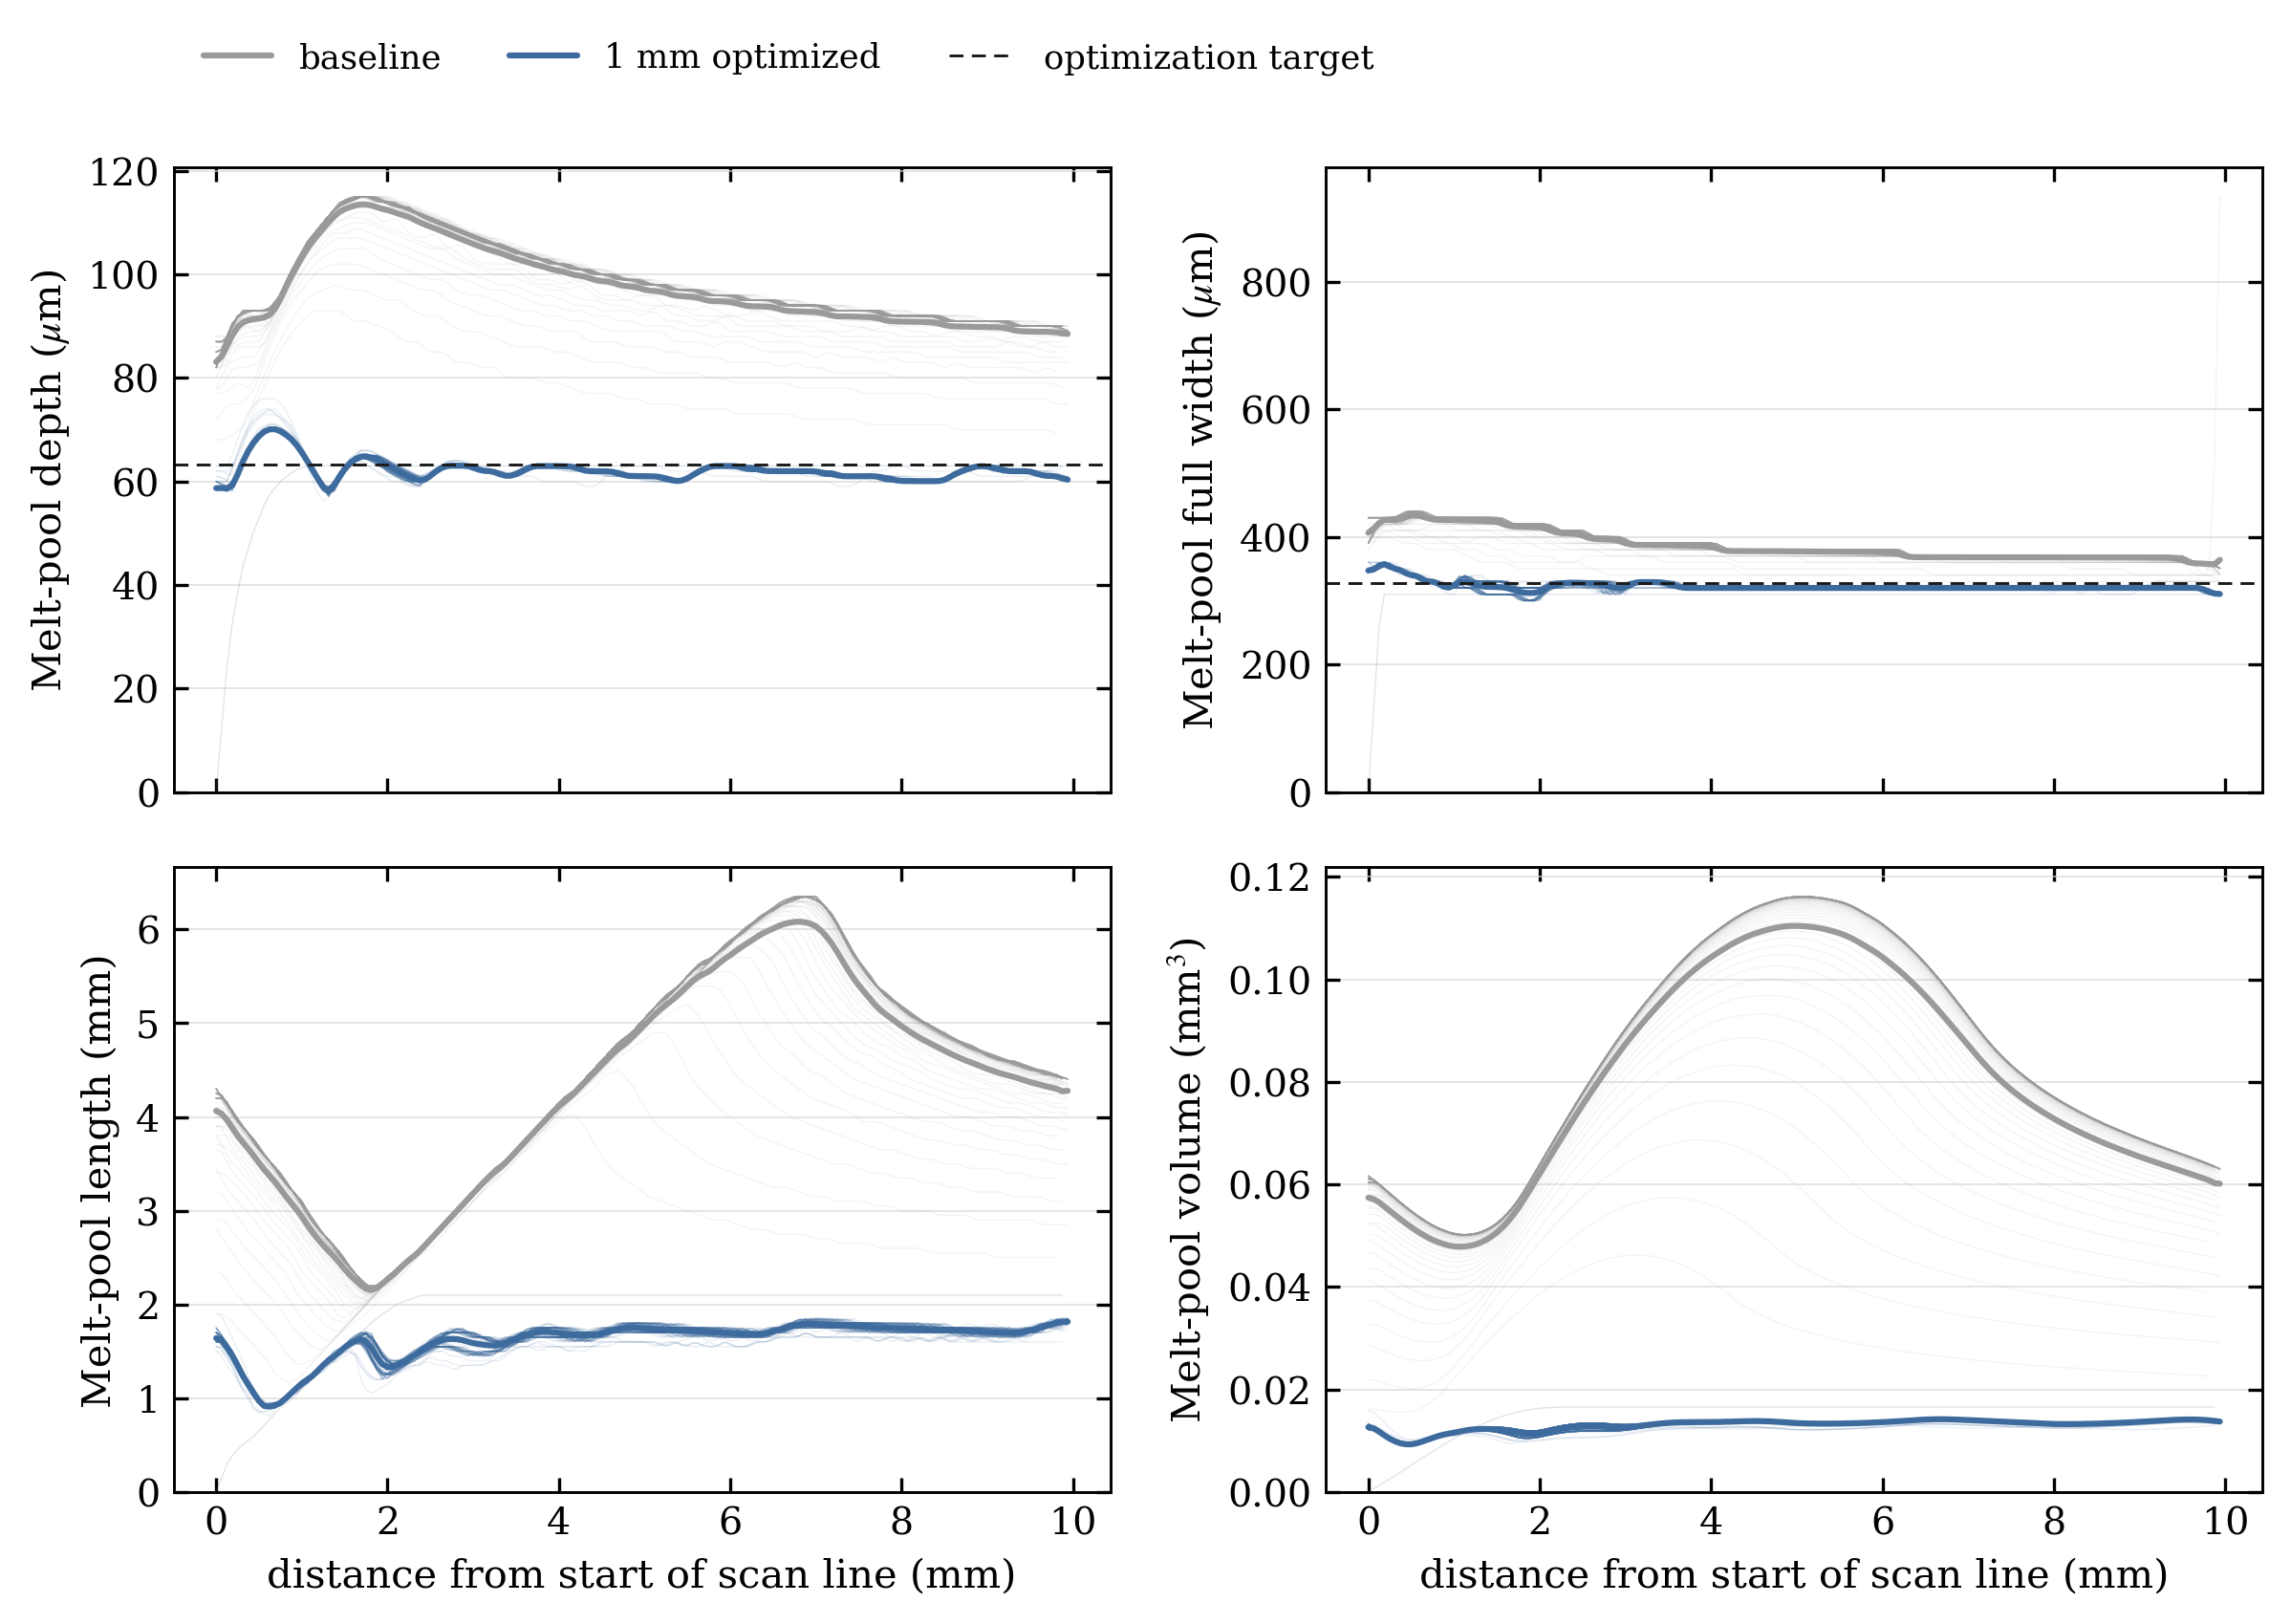
\includegraphics[width=0.95\textwidth]{square_profiles_zero.png}
\caption{The same zero-dwell data folded per line: all 101 lines overlaid
against position along the line (light curves), with the per-case mean
(bold). After the $\sim$15-line startup the bundles are nearly
one-dimensional --- line-to-line variation is essentially eliminated by the
statistically steady process and, for the optimized schedule, the remaining
imperfection is the repeatable within-line structure: the inherited pool at
position 0, its die-off near 1\,mm, and the development hump at
1.5--3.5\,mm that the per-segment controller cannot resolve.}
\label{fig:square-profiles}
\end{figure}

\paragraph{The triangle.} The same machinery (environment-selected
geometry) runs the triangle raster: 131 controlled segments over 87
shrinking lines, same target. Its minimal worst-case dwell is
$1.672$\,ms/turn with the \emph{binding turn near the apex} (\#79) --- that
global dwell takes the 149\,ms continuous path to 290\,ms ($+94\%$ build
time, versus $+26\%$ for the square), which is the quantitative case for
the adaptive per-turn dwell below. At nominal power the shrinking lines
drive the pool from the $164\,\mu$m single-track half-width at the base to
an $875\,\mu$m lake near the apex; on whole-build statistics the optimizer
cuts the pool-volume fluctuation $7\times$ at zero dwell
($0.113\pm0.048 \to 0.022\pm0.007$\,mm$^3$; beam-on depth
$116\pm21 \to 68\pm9\,\mu$m, fusion-depth map $111\pm25 \to 65\pm12\,\mu$m)
and $4\times$ with the dwell. The residual variation concentrates entirely
at the apex, where the bound-pinning diagnostic localizes the physics:
segment-end CVs are square-quality over the body (w/d $0.2$--$0.3\%$,
lines 0--69) but degrade over the last $\sim$17 lines, and the two policies
fail in \emph{opposite} directions. With the dwell (solidified starts), the
$0.07$\,mm tip line pins at \textbf{maximum power} (450\,W) yet remains
$21\,\mu$m short of target depth --- $23\,\mu$s of beam time cannot develop
a pool, and the physical fix is \emph{slowing down}. At zero dwell, lines
80--83 pin $\sigma$ at its floor and lines 84--86 pin at \textbf{minimum
power} (8\,W) with the pool still at or above target width --- pure
inherited melt, and the fix is \emph{waiting} (dwell) or again slowing
down. Between them, the apex brackets exactly the two control degrees of
freedom developed next.

\begin{figure}[h]
\centering
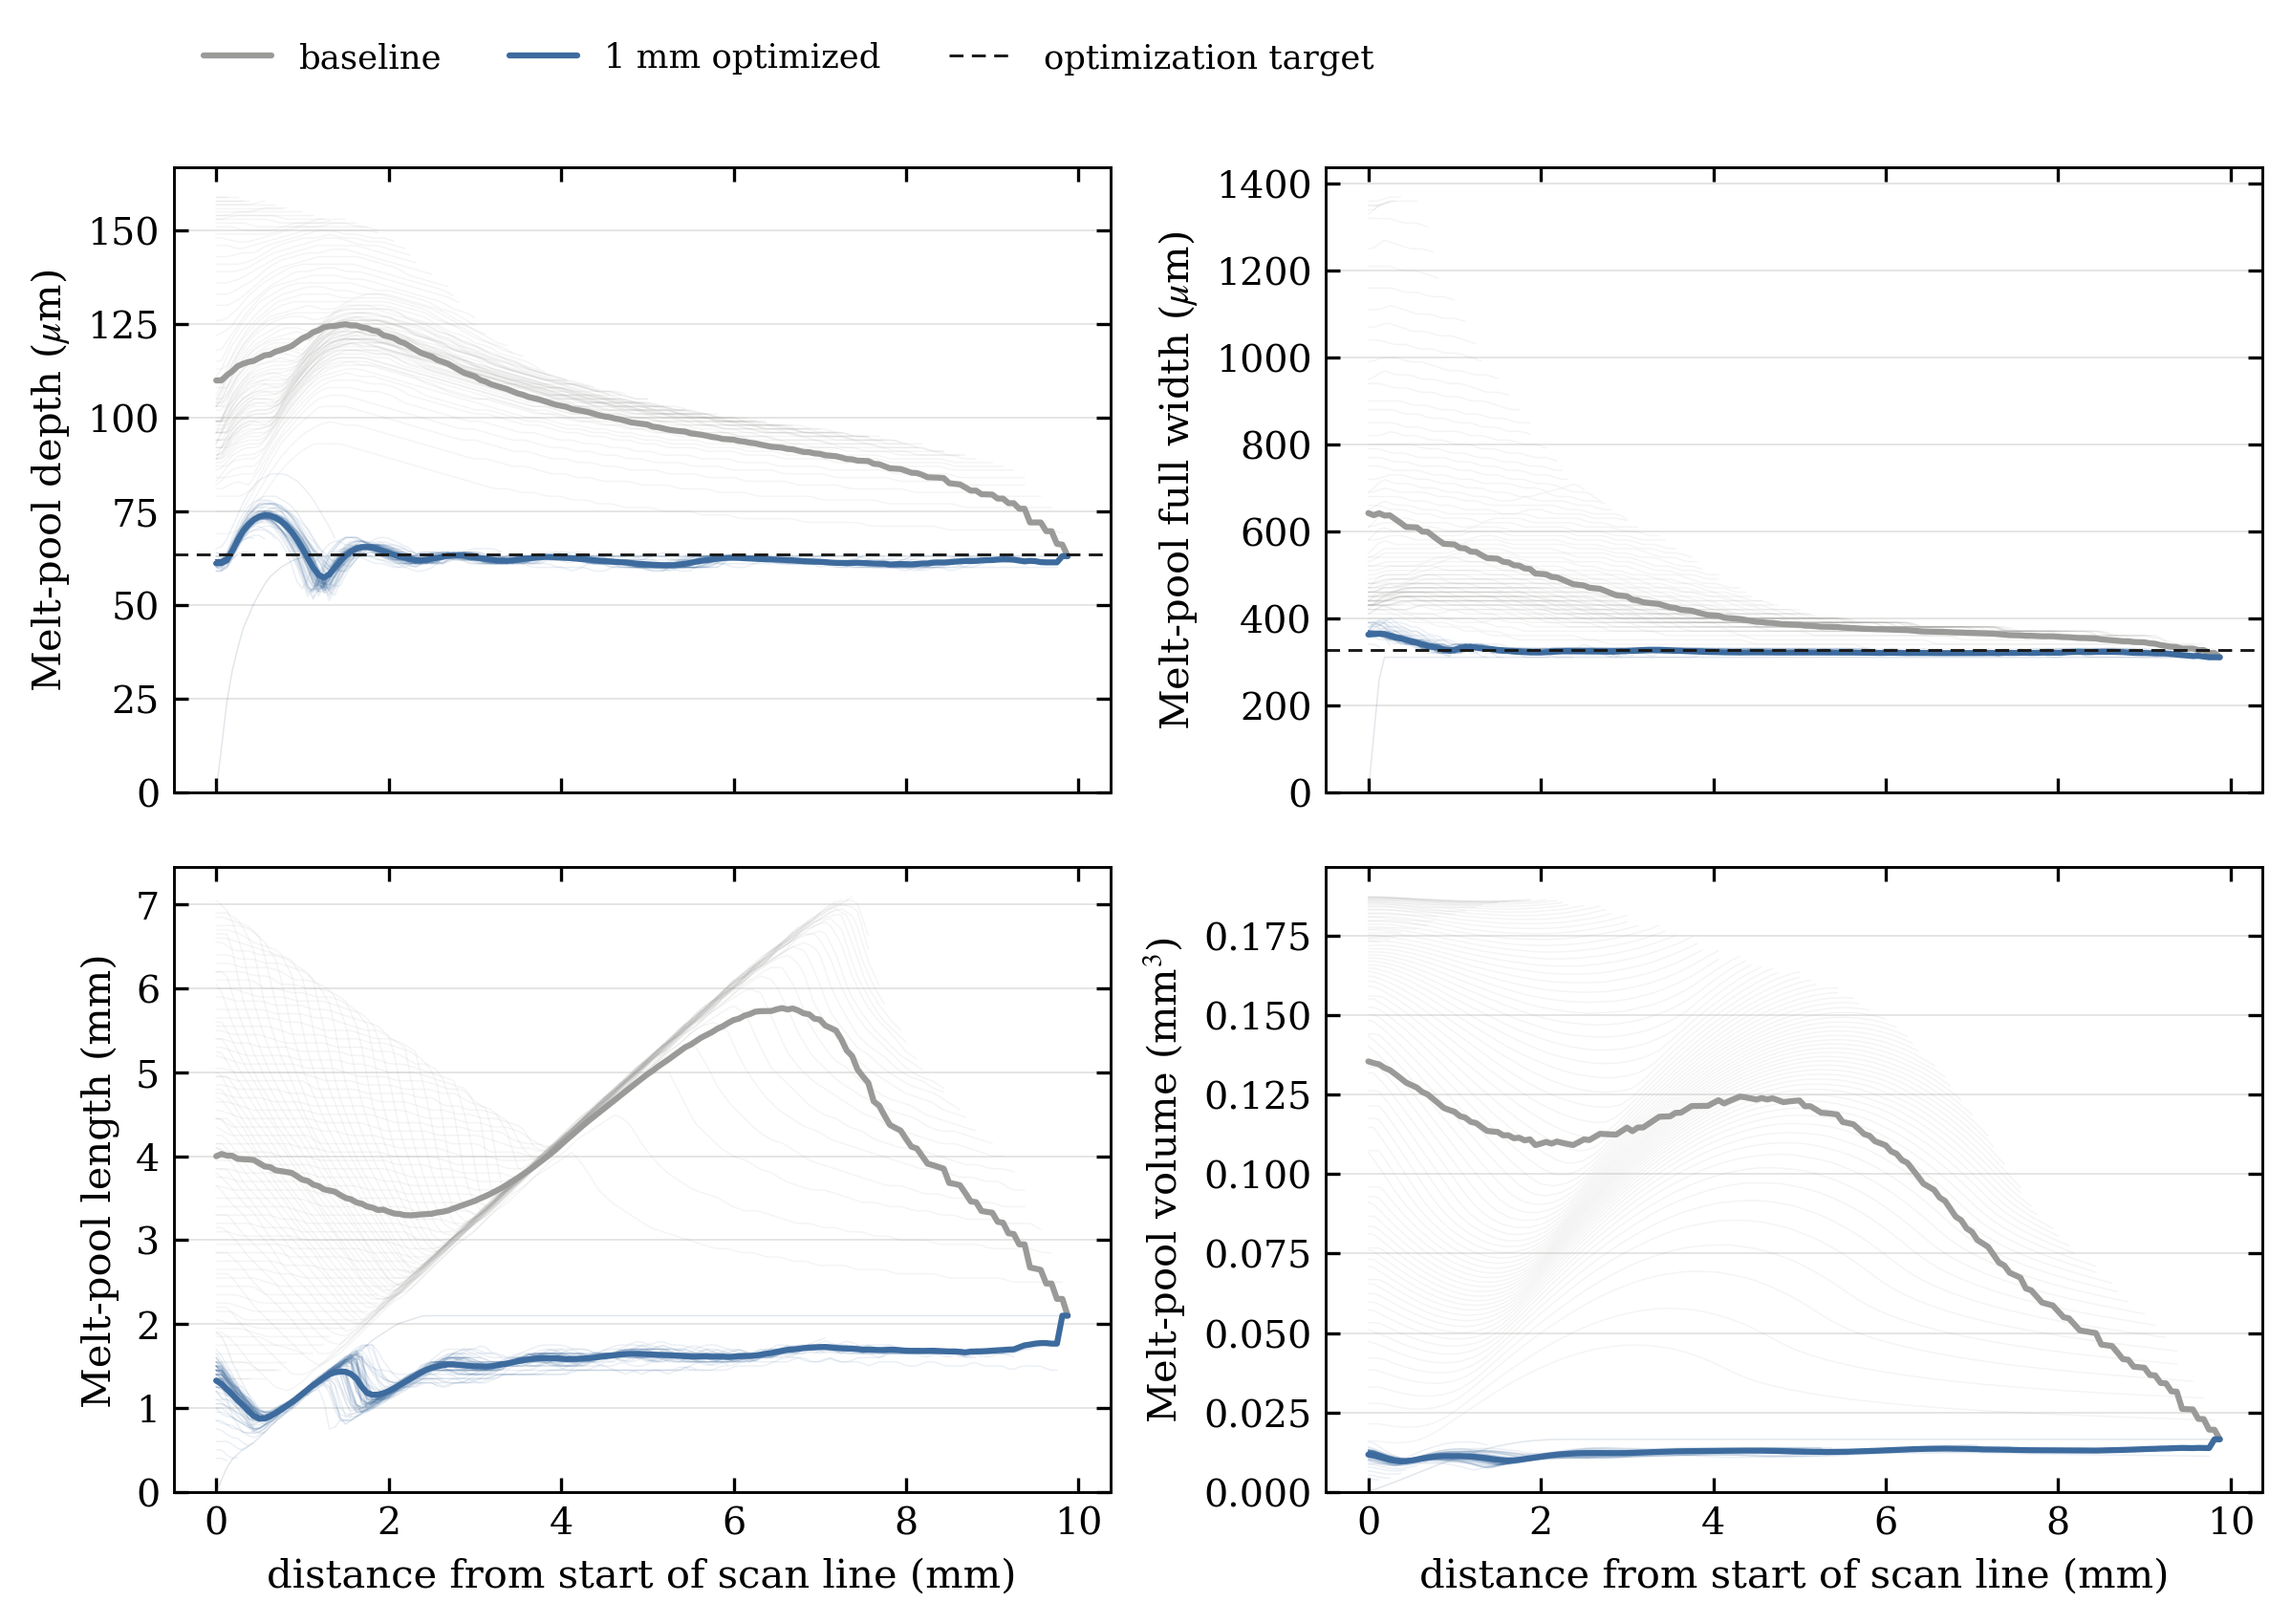
\includegraphics[width=0.95\textwidth]{triangle_profiles_zero.png}
\caption{The zero-dwell triangle folded per line (all 87 lines): the
unoptimized fan --- every line a different length, the pool deepening and
widening toward the apex --- collapses onto the target band under the
optimized schedule, with the apex lines carrying the residual variation
that power and beam width cannot remove.}
\label{fig:triangle-profiles}
\end{figure}

\begin{figure}[h]
\centering
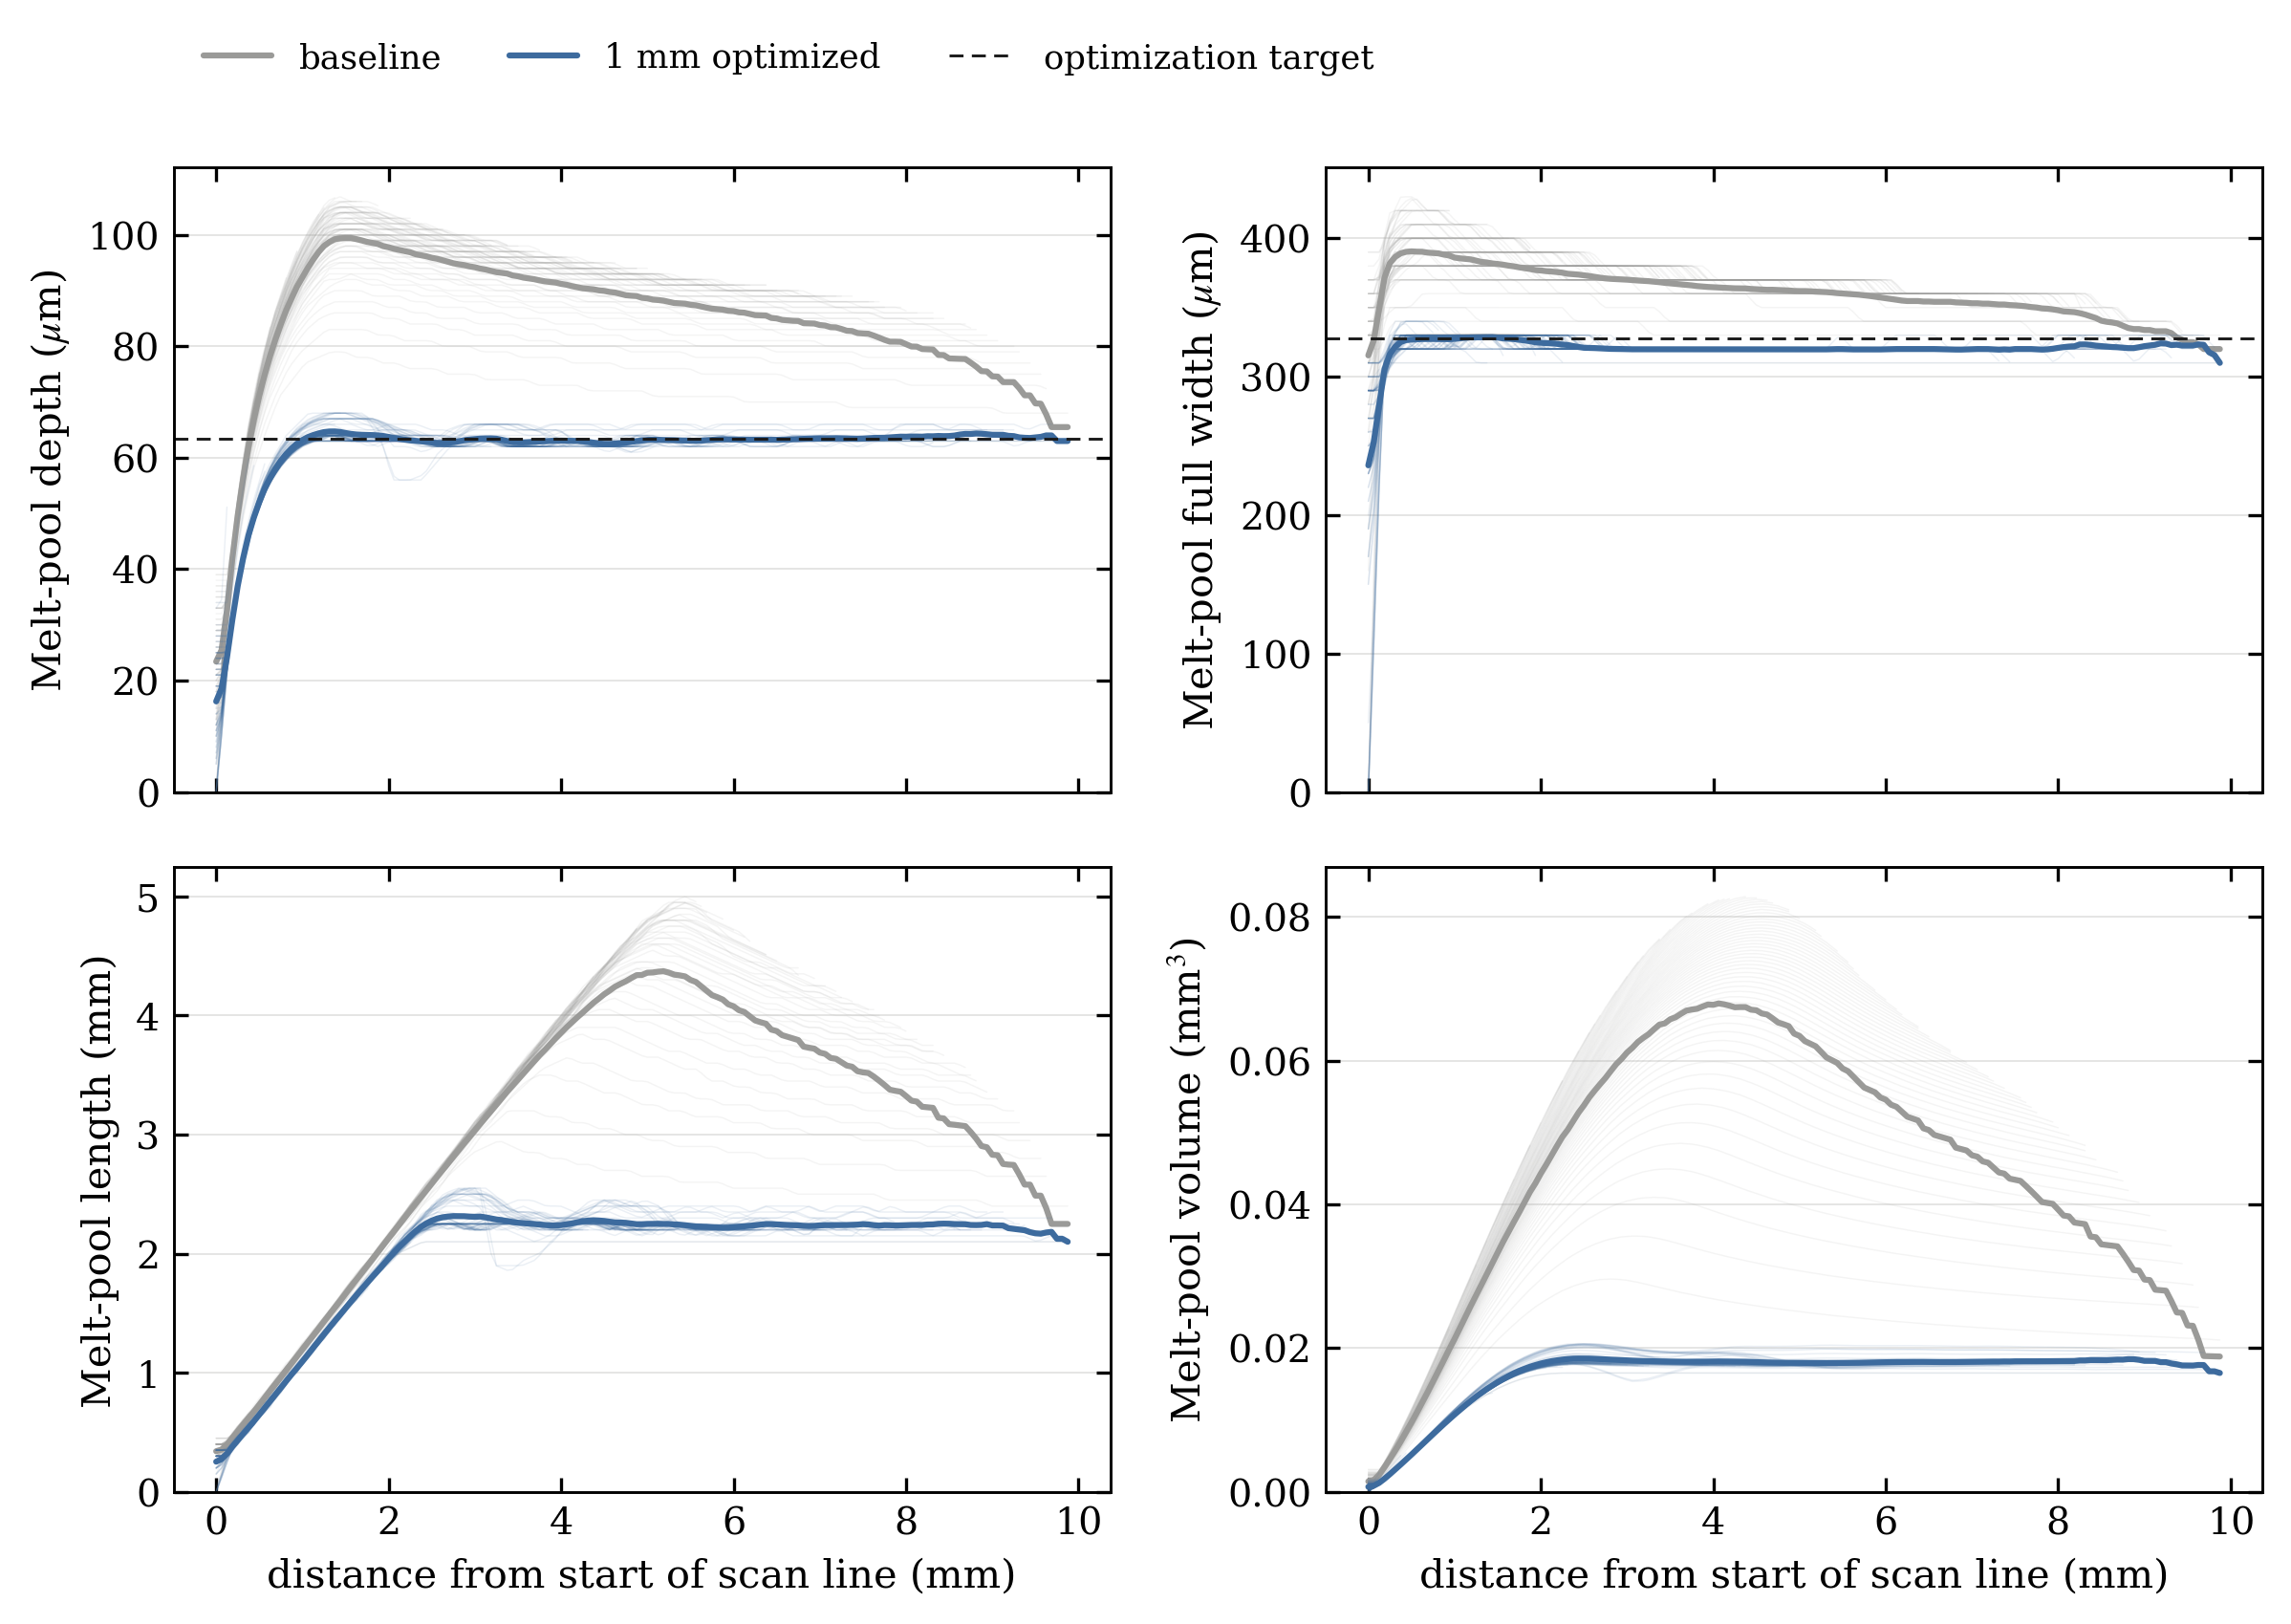
\includegraphics[width=0.95\textwidth]{triangle_profiles_dwell.png}
\caption{The minimal-dwell triangle folded per line: with solidified starts
every pool is reborn from cold ground, so the profiles carry the
development ramp once per line; the optimized bundle rides the target until
the shortest apex lines, whose pools cannot develop within the available
beam time even at the 450\,W power ceiling.}
\label{fig:triangle-profiles-dwell}
\end{figure}

\section{Limitations and next steps}

\begin{itemize}
  \item \textbf{Velocity as a control.} Scan speed is fixed at the raster
        speed. Velocity is the missing degree of freedom whenever $\sigma$
        pins at its lower bound and the depth-to-width ratio cannot be
        restored. The exact sensitivity $\partial_v T$ is now implemented and
        validated as the sixth OTI direction (Section~\ref{sec:velderiv});
        what remains is wiring it into the per-segment solve. Because $v$ and
        $Q$ move the pool in nearly opposite directions in $(w,d)$ space ---
        both dominated by depth --- the natural formulation is time-optimal
        (maximize $v$ subject to $(w,d)=(w^\ast,d^\ast)$, with $Q,\sigma$ as
        feasibility controls) rather than adding $v$ as a third co-regulated
        knob; power saturating at its upper bound is the expected binding
        constraint on the achievable speed-up.
  \item \textbf{First-order control model.} The $2\times2$ Jacobian is exact
        but local; strong nonlinearity near bounds is handled by damping
        rather than curvature. Second-order OTI jets
        (\texttt{otinum<M,2>}) would provide exact Hessians at the same
        single-run structure if a trust-region Newton on the merit function
        ever becomes necessary.
  \item \textbf{Per-segment greedy horizon.} Each segment is solved given a
        frozen history; there is no look-ahead. A receding-horizon variant
        would re-use the same OTI Jacobians.
  \item \textbf{Adaptive dwell.} The global worst-case dwell is wasteful:
        it is sized by the single binding turn ($+26\%$ build time on the
        square; nearly $2\times$ on the triangle, where the apex binds).
        Since a dwell simply ages all previously deposited heat,
        $\partial T/\partial t_{\mathrm{dwell}}$ is seedable exactly like
        the other OTI directions, and a per-turn Newton solve on the
        solidification criterion would replace the current
        bisection-by-resimulation with one or two simulations per turn ---
        the same trick this whole document is about, applied to the
        feasibility constraint instead of the target.
\end{itemize}

\appendix
\section{Derivation of the velocity sensitivity}
\label{app:vel}

The spatial and power derivatives (\S\ref{sec:oti}) follow by differentiating
the integrand of the moving-source solution~\eqref{eq:nguyen} --- the paper's
Eq.~(2) --- over a \emph{fixed} integration domain, exactly as its Appendix~B
obtains the thermal gradients $G_{x,y,z}$. Velocity is different: it appears
nowhere in the integrand, only in the \emph{parametrization} of the integral,
so the domain itself moves. We carry the derivation out here, both to justify
the closed-form reference of \S\ref{sec:velderiv} and to show, in the open,
what the OTI arithmetic does silently.

Write the scan-end field as an integral over deposition time $t'$,
\begin{equation}
  T - T_0 = A \int_0^{t_{\mathrm{end}}} K(t')\,\dd t',
  \quad
  K = \frac{\exp\!\big(-3\textstyle\sum_i r_i^2/\phi_i\big)}{\sqrt{\phi_x\phi_y\phi_z}},
  \quad
  \phi_i = 12\alpha\,(t_{\mathrm{end}}-t') + \sigma_i^2,
  \label{eq:app-T}
\end{equation}
with $A = 2\eta Q/\rho c\,(\pi/3)^{3/2}$, $r_i(t') = x_{p,i} - x_{b,i}(t')$ the
offset from the moving beam, and $t_{\mathrm{end}}-t'$ the conduction time.
Perturb the speed $v$ of the \emph{last} segment only, at fixed path geometry;
both effects funnel through its duration $\Delta t = L/v$ ($L$ its fixed
length):
\begin{enumerate}
  \item the observation is the scan end, so $t_{\mathrm{end}} = t_{N-1} +
        \Delta t$, with $t_{N-1}$ (the instant the segment begins) frozen by
        the history;
  \item within the segment the beam is at fixed fraction $\xi\in[0,1]$ of its
        \emph{path}, $x_b = x_{N-1} + \xi L$, but \emph{deposited} at
        $t' = t_{N-1} + \xi\Delta t$ --- the deposition times stretch with
        $\Delta t$.
\end{enumerate}
Point~(2) is why one may not differentiate~\eqref{eq:app-T} under a fixed $t'$:
the map from physical position to deposition time depends on $v$ (naive Leibniz
at fixed $t'$ omits $\partial x_b/\partial\Delta t$, since at fixed absolute
time a slower beam is less far along). We split at $t_{N-1}$ and treat each
piece on its natural, $v$-independent domain. Using
$\partial K/\partial\phi_i = K\,(3r_i^2/\phi_i^2 - 1/2\phi_i)$, abbreviate
\begin{equation}
  S(t') \equiv \sum_i \left(\frac{3 r_i^2}{\phi_i^2} - \frac{1}{2\phi_i}\right),
  \qquad\text{so}\qquad
  \frac{\partial K}{\partial \Delta t} = 12\alpha\,w\,K\,S
  \label{eq:app-S}
\end{equation}
whenever a change in $\Delta t$ shifts every $\phi_i$ by the common amount
$12\alpha\,w\,\dd\Delta t$.

\paragraph{History, $0 \le t' \le t_{N-1}$.} The limits and deposition times
are fixed; $\Delta t$ enters only through $t_{\mathrm{end}}$ in
$\phi_i = 12\alpha(t_{N-1}+\Delta t - t') + \sigma_i^2$, so $w=1$ and
\begin{equation}
  \frac{\dd}{\dd\Delta t}\!\int_0^{t_{N-1}}\! K\,\dd t'
  = 12\alpha \int_0^{t_{N-1}} K\,S\,\dd t' \;\equiv\; H .
  \label{eq:app-H}
\end{equation}
Every history node's Gaussian broadens because the field is observed a little
later --- the $t_{\mathrm{shift}}$ channel.

\paragraph{Last segment, $t_{N-1}\le t' \le t_{\mathrm{end}}$.} Change to the
fixed variable $\xi$: $t' = t_{N-1}+\xi\Delta t$, $\dd t' = \Delta t\,\dd\xi$,
whence $t_{\mathrm{end}}-t' = (1-\xi)\Delta t$ and $\phi_i = 12\alpha(1-\xi)
\Delta t + \sigma_i^2$, with $v$-independent limits. Differentiating the
fixed-limit form splits into a Jacobian and an integrand term,
\begin{equation}
  \frac{\dd}{\dd\Delta t}\Big[\Delta t \!\int_0^1\! \tilde K\,\dd\xi\Big]
  = \underbrace{\int_0^1 \tilde K\,\dd\xi}_{W}
  \;+\; \underbrace{\Delta t\!\int_0^1 \frac{\partial\tilde K}{\partial\Delta t}\,\dd\xi}_{C},
\end{equation}
where $W$ is the weight growing because the segment lasts longer, and $C$ uses
$w = (1-\xi)$ in~\eqref{eq:app-S} (a node early in the segment ages more when it
is stretched; the node at the observation instant, $\xi=1$, not at all).
Restored to $t'$,
\begin{align}
  W &= \frac{1}{\Delta t}\int_{t_{N-1}}^{t_{\mathrm{end}}} K\,\dd t', \label{eq:app-W}\\
  C &= \frac{12\alpha}{\Delta t}\int_{t_{N-1}}^{t_{\mathrm{end}}}
        (t_{\mathrm{end}}-t')\,K\,S\,\dd t'. \label{eq:app-C}
\end{align}

\paragraph{Result.} With $\dd\Delta t/\dd v = -L/v^2$,
\begin{equation}
  \frac{\dd T}{\dd v} = -\frac{L}{v^2}\,A\,(H + W + C),
  \label{eq:app-dTdv}
\end{equation}
the three integrals evaluated by the closed-form reference of
\S\ref{sec:velderiv}: $W$ and $C$ the last-segment weight and conduction-time
channels, $H$ the history channel.

Forward-mode AD never forms \eqref{eq:app-H}--\eqref{eq:app-C}. It seeds the
single scalar $\Delta t = L/v$ with $\partial\Delta t/\partial v = -L/v^2$, and
facts~(1)--(2) enter as the two node dressings of \S\ref{sec:velderiv}:
current-segment node conduction times and weights carry $k = \Delta t/\Delta t_0$,
history-node conduction times carry $t_{\mathrm{shift}} = \Delta t - \Delta
t_0$. Propagating those through $K$ node-by-node and summing --- one pass ---
reproduces \eqref{eq:app-dTdv} term for term: the derivative of $k$ feeds $W$
(its weight part) and $C$ (its conduction part), and that of $t_{\mathrm{shift}}$
feeds $H$. The derivation above is only the closed-form view of the chain rule
the hypercomplex numbers carry automatically.

\begin{thebibliography}{9}
\bibitem{stump2019}
B.~Stump and A.~Plotkowski,
``An adaptive integration scheme for heat conduction in additive
manufacturing,''
\emph{Applied Mathematical Modelling} \textbf{75} (2019) 787--805.
doi:10.1016/j.apm.2019.07.008.

\bibitem{nguyen1999}
N.~T. Nguyen, A.~Ohta, K.~Matsuoka, N.~Suzuki, and Y.~Maeda,
``Analytical solutions for transient temperature of semi-infinite body
subjected to 3-D moving heat sources,''
\emph{Welding Journal} \textbf{78} (1999) 265s--274s.

\bibitem{cppoti}
\texttt{cpp\_oti\_lib}: header-only static order-truncated imaginary (OTI)
numbers for C++ (\texttt{oti::otinum<M,N,T>}), used here as the 3DThesis
scalar type with $M=5$ directions at order $N=1$.
\end{thebibliography}

\end{document}
